\chapter{Utvrđivanje relativne i apsolutne lokacije u zatvorenom prostoru}

Tehnologije navigacije i pozicioniranja koje se oslanjaju na udaljene satelite (poput GPS i GNSS tehnologija) nisu pogodne za korištenje u zatvorenim prostorima iz razloga što njihove signale apsorbiraju i reflektiraju krovovi, zidovi i ostali objekti u okolini. 
Iz istih razloga određivanje lokacije preko mobilnih signala, odnosno preko radio tornjeva nije moguće. 
\\
Stoga su za utvrđivanje lokacije u zatvorenom prostoru potrebni sasvim novi i drugačiji pristupi problemu te shodno tome, sasvim nove metode određivanja lokacije. 
Zbog ogromnog porasta pristupačnosti i popularnosti pametnih telefona, posljednjih nekoliko godina sve je veća potražnja za nekakvim pouzdanim rješenjem problema. 
Kako ne postoji nikakav \textit{de facto} standard, gotovo sva ponuđena rješenja su međusobno različita i koriste cijeli niz različitih tehnologija, od optičkih (npr. kamera uređaja) i radio (npr. signali obližnje bežične mreže) skroz do akustičnih tehnologija.
\\

Vjerojatno najznačajniji uspjeh je postignut sa praćenjem signala kojega odašilje obližnja bežična Wi-fi mreža. 
Velika prednost ove metode je značajan porast bežičnih pristupnih točaka na koje se mobilni i drugi uređaji mogu spojiti. 
Da bi se ovom metodom odredila lokacija uređaja potrebno je na neki način mapirati dotičnu pristupnu točku te zatim na temelju jakosti primljenog signala utvrditi poziciju mobilnog uređaja u odnosu na nju. 
Parametri mapiranja uključuju apsolutnu poziciju, SSID\footnote{\textit{service set identification}} i MAC\footnote{\textit{media access control address}} adresu pristupne točke (tj. WLAN uređaja). 
Neke od poznatijih web aplikacija poput WeFi\footnote{\url{http://www.wefi.com/maps/}} i WiGLE\footnote{\url{https://wigle.net}} sadrže više od sto milijuna mapiranih bežičnih pristupnih točaka. 
\\

\begin{figure}
    \centering
    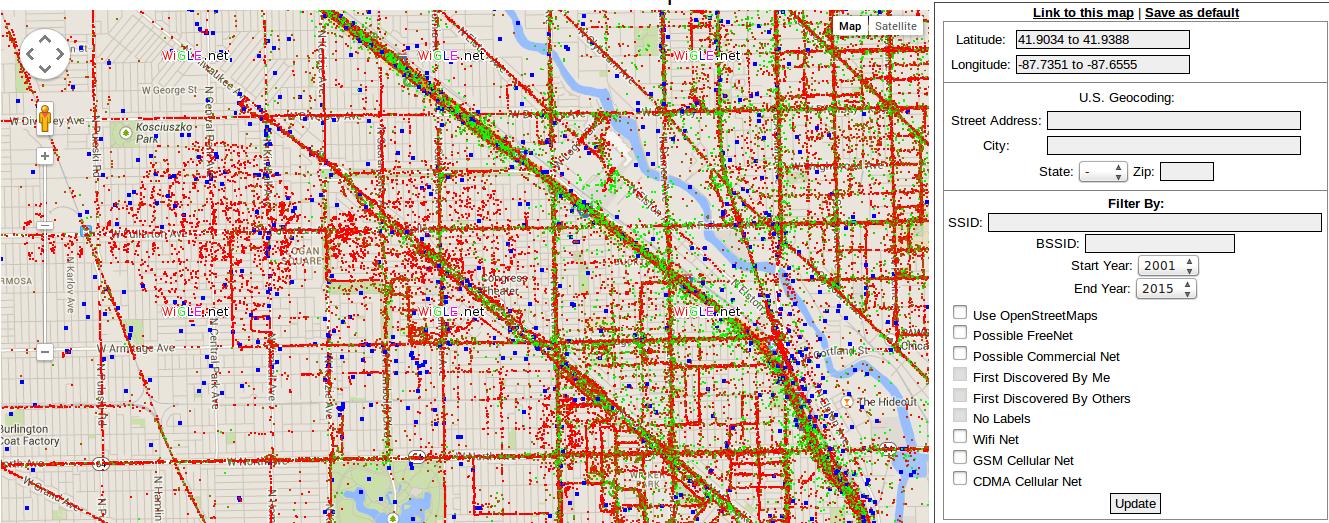
\includegraphics[scale=0.3]{pictures/WiGLE}
    \caption{WIGLE} % TODO caption
\end{figure}

Uz navigaciju i pozicioniranje pomoću Wi-fi mreža, dosta su popularne metode koje se služe tehnikama proširene i virtualne stvarnosti te tehnikama strojnog učenja, raspoznavanja uzoraka i računalnog vida. 
Jedna od popularnijih tehnika proširene i virtualne stvarnosti je korištenje posebnih oznaka (markera) kojega kamera mobilnog uređaja može prepoznati u prostoru. 
Vezano za metode strojnog učenja, raspoznavanja uzoraka i računalnog vida vjerojatno najistaknutiji i najambiciozniji projekt je projekt Tango\footnote{\url{https://www.google.com/atap/projecttango/}} kojega razvija tehnološki gigant Google. 
Cilj projekta je ponuditi rješenje koje će korištenjem kamere i ostalih senzora mobilnog uređaja nuditi pomoć pri navigaciji, pozicioniranju i prepoznavanju okoline, odnosno 3D mapiranje, u zatvorenom i otvorenom prostoru. 
Unatoč tome što je projekt još u ranoj fazi razvoja, razvojni tim je ostvario vidljiv napredak te su prvi prototipovi mobilnih uređaja već dostupni partnerima koji sudjeluju u razvoju.

\begin{figure}[H]
    \centering
    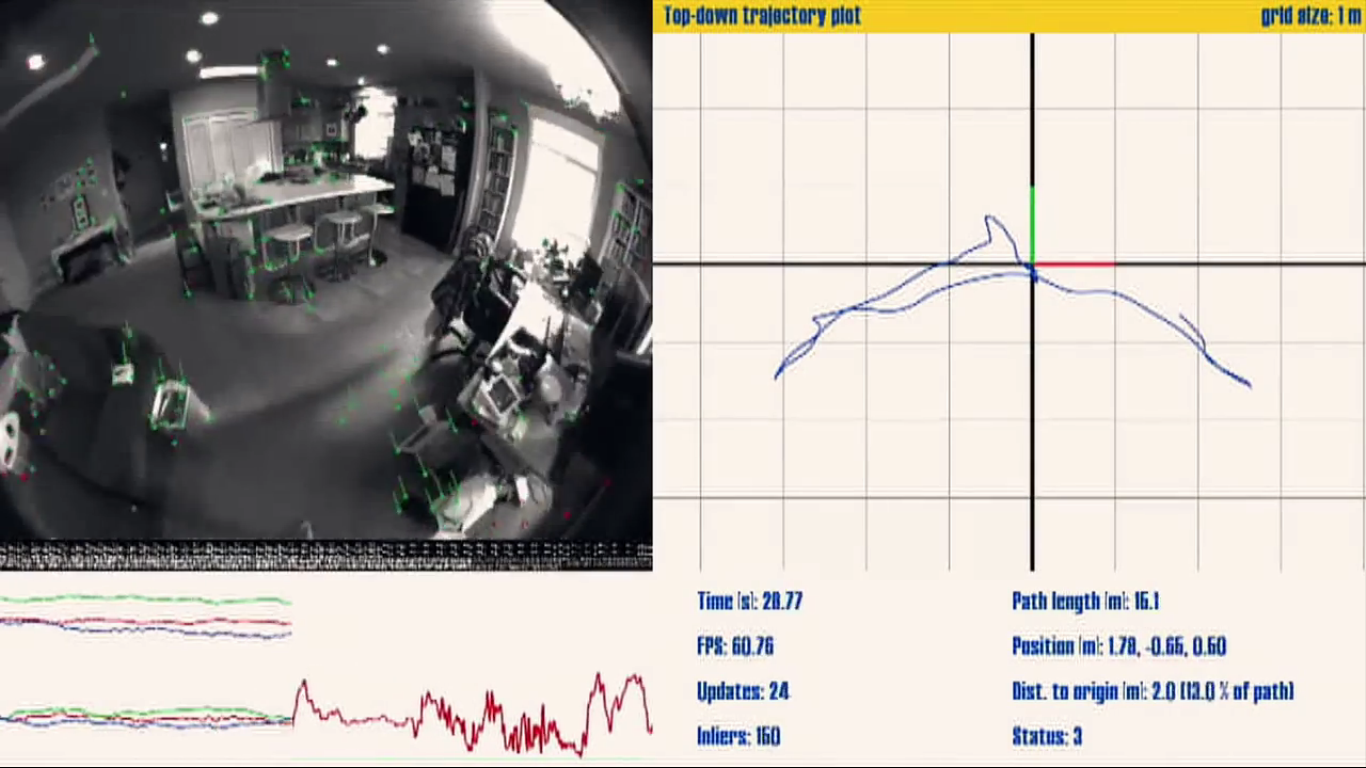
\includegraphics[scale=0.24]{pictures/tango1}
    \caption{Project Tango 1}
\end{figure}

\begin{figure}[H]
    \centering
    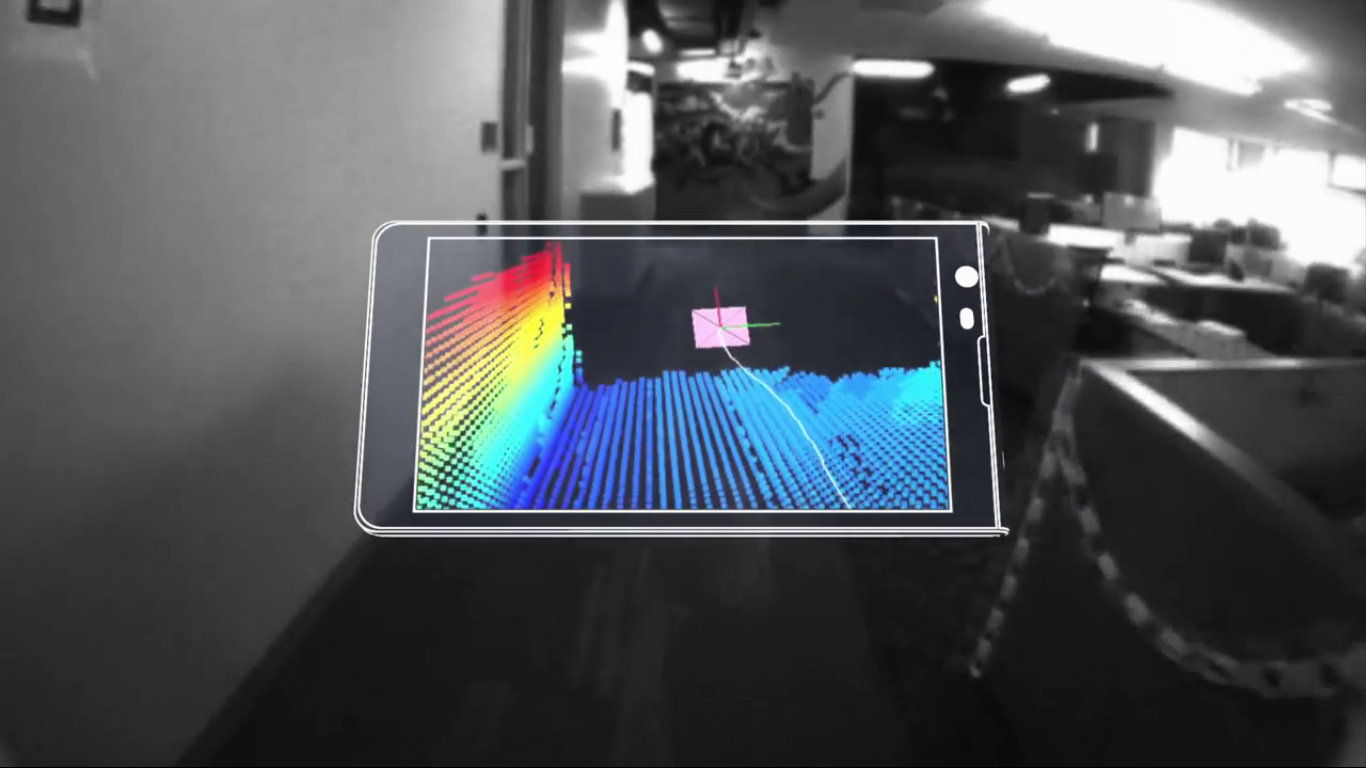
\includegraphics[scale=0.24]{pictures/tango2}
    \caption{Project Tango 2}
\end{figure}
%TODO referencirati youtube video u captionu

\section*{Utvrđivanje relativne udaljenosti od odašiljača}

blabla neki tekst.

%TODO postupak mjerenja, što sve treba, kako mjeriti, poteškoće
%TODO postupci: matematički, best fit curve, neuronska mreža i poteškoće, spomeniti genetsko programiranje
%TODO mjerenja udaljenosti
%TODO zaključak

\begin{table}[H]
    \centering
    \caption{Rezultat mjerenja signala u zatvorenom prostoru}
    \label{tbl:indoor}
	\begin{tabular}{|c|cccc||cccc|}%||cccc}
	\cline{2-9}
	\multicolumn{1}{!{\vrule width 0pt}c!{\vrule width 1pt}}{} & \multicolumn{4}{c||}{Beacon1} & \multicolumn{4}{c|}{Beacon2} \\ %& \multicolumn{4}{c}{Beacon3} \\ 
	\hline 
	Udaljenost & $\mu_{RSSI}$ & $\sigma_{RSSI}$ & $min_{RSSI}$ & $max_{RSSI}$ & $\mu_{RSSI}$ & $\sigma_{RSSI}$ & $min_{RSSI}$ & $max_{RSSI}$ \\ %& $\mu_{RSSI}$ & $\sigma_{RSSI}$ & $min_{RSSI}$ & $max_{RSSI}$ \\ 
	\hline 
	$0.5$ & $-81.075$ & $2.426$ & $-88$ & $-74$ & $-65.165$ & $2.546$ & $-76$ & $-56$ \\ %& -89.550 & 3.526 & -98 & -83 \\ 
	$1.0$ & $-80.320$ & $2.799$ & $-86$ & $-76$ & $-66.250$ & $2.316$ & $-73$ & $-59$ \\ %& -90.895 & 2.101 & -96 & -86 \\ 
	$1.5$ & $-75.575$ & $3.298$ & $-80$ & $-70$ & $-62.695$ & $4.324$ & $-69$ & $-57$ \\ %& -91.350 & 3.162 & -101 & -86 \\ 
	$2.0$ & $-73.990$ & $2.558$ & $-79$ & $-68$ & $-58.750$ & $1.982$ & $-62$ & $-53$ \\ %& -91.695 & 2.134 & -99 & -86 \\ 
	$2.5$ & $-78.725$ & $0.907$ & $-81$ & $-74$ & $-63.595$ & $0.875$ & $-66$ & $-59$ \\ %& -89.630 & 1.583 & -99 & -86 \\ 
	$3.0$ & $-82.470$ & $4.053$ & $-91$ & $-74$ & $-67.810$ & $2.619$ & $-73$ & $-62$ \\ %& -93.385 & 2.156 & -100 & -88 \\ 
	$3.5$ & $-81.685$ & $2.892$ & $-87$ & $-77$ & $-71.620$ & $3.537$ & $-80$ & $-65$ \\ %& - & - & - & - \\ 
	$4.0$ & $-83.115$ & $1.903$ & $-88$ & $-77$ & $-68.720$ & $2.000$ & $-73$ & $-65$ \\ %& - & - & - & - \\ 
	$4.5$ & $-91.125$ & $3.057$ & $-98$ & $-85$ & $-74.975$ & $3.065$ & $-81$ & $-68$ \\ %& - & - & - & - \\ 
	$5.0$ & $-88.705$ & $2.198$ & $-93$ & $-83$ & $-72.445$ & $3.485$ & $-78$ & $-65$ \\ %& - & - & - & - \\ 
	$5.5$ & $-88.935$ & $3.487$ & $-97$ & $-83$ & $-79.920$ & $6.883$ & $-93$ & $-68$ \\ %& - & - & - & - \\ 
	$6.0$ & $-92.450$ & $2.399$ & $-99$ & $-87$ & $-82.175$ & $5.896$ & $-98$ & $-71$ \\ %& - & - & - & - \\ 
	$6.5$ & $-93.610$ & $1.691$ & $-99$ & $-90$ & $-74.085$ & $2.977$ & $-80$ & $-68$ \\ %& - & - & - & - \\ 
	$7.0$ & - & - & - & - & $-71.700$ & $2.858$ & $-77$ & $-65$ \\ %& - & - & - & - \\ 
	$7.5$ & - & - & - & - & $-76.065$ & $2.241$ & $-80$ & $-71$ \\ %& - & - & - & - \\ 
	$8.0$ & - & - & - & - & $-78.295$ & $4.926$ & $-91$ & $-71$ \\ %& - & - & - & - \\ 
	\hline 
	\end{tabular}
\end{table}


\section*{Utvrđivanje apsolutne lokacije}
%TODO općenito o utvrđivanju apsolutne lokacije

\subsection*{Triangulacija}

Postupak triangulacije
%TODO objasniti postupak triangulacije
%TODO matematički postupak kod triangulacije
%TODO iBeacon i triangulacija

\subsection*{Trilateracija}
%TODO objasniti postupak trilateracije
%TODO matematički postupak trilateracije
%TODO iBeacon i trilateracija